\documentclass[10pt,a4paper]{article}
\usepackage[utf8]{inputenc}
% \usepackage[cp1250]{inputenc}
\usepackage{amsmath}
\usepackage{amsfonts}
\usepackage{amssymb}
\usepackage{graphicx}

\usepackage{listings} % formatting source code
\newcommand{\HRule}{\rule{\linewidth}{0.5mm}}

\begin{document}
\begin{titlepage}
\begin{center}


\textsc{\LARGE Wrocław University of Technology}\\[1.5cm]

\textsc{\Large Advanced databases}\\[0.5cm]

% Title
\HRule \\[0.4cm]
{ \huge \bfseries Performance in MySQL: indexes and caching \\[0.4cm] }

\HRule \\[1.5cm]

% Author and supervisor
%\begin{minipage}{0.4\textwidth}
%\begin{flushleft} \large
%\emph{Author:}\\
%Artur \textsc{Zochniak} (184725)
%\end{flushleft}
%\end{minipage}
\begin{minipage}{0.4\textwidth}
\begin{flushright} \large
\emph{Author:} \\
Artur \textsc{Zochniak} (184725)
\end{flushright}
\end{minipage}

\vfill

% Bottom of the page
{\large \today}

\end{center}
\end{titlepage}

\newpage

\section{Introduction}
This document shows how database behaviour is determined by number of rows in tables. 
Tests will measure database performance in following axises: 
\begin {itemize}
\item number of entities in database (in this case, example data are in database representing cinema, therefore assumption is entities - in this case hours of shows in rooms - are equally distributed - in other words - every room has the same number of shows in databse), 
\item whether index is added to this table, 
\item whether caching is turned on. 
\end{itemize}

\section{Description of database}
For simplicity, only used tables are listed in this chapter. 
Database consists of following tables: 
\begin {itemize}
\item rooms - represents rooms in cinema(s), 
\item room\_schedules - represents shows which are planned for each room, 
\item films - stores informations about whole variety of movies which are showed in all cinemas, in all rooms during all times. 
\end {itemize}

\section{Generating random data}
In order to test performance of database at least few test cases are needed. Database is such a fast utility that for noticing any significant differences in performance, there have to be thousands of records. For this purpose generation of random data is required. 
Generation could be performed outside MySQL, for example in some imperative language, but since this document is about MySQL, generation of random data is performed within SQL, too.  

\section{Random list of rooms}

In order to generate data, list of rooms and movies (films) is required. The goal is to limit number of generated rows to only few from two reasons: 
\begin{itemize}
\item it is easier to develop such a SQL query, if there are no thousands of rows, 
\item having such a limitation of rows implementation, it is possible to flexibly change number of generated rows, which is crucial in having possibility of comparing how database behaves in different cases from the point of view of amount of entities in database. 
\end{itemize}
Intuitively it should be possible to generate data with simple, for example, IN statement, but MySQL will throw an exception in this case saying that it is impossible to use LIMIT along with IN/ALL/ANY/SOME. If it is not possible to use limit in subqueries, another way of putting LIMIT in query is in temporary table which is created as a consequence of every JOIN statement. 




Query: select * from room r   where id in (select id from room  limit 3) LIMIT 0, 1000    
Error Code: 1235. This version of MySQL doesn't yet support 'LIMIT \& IN/ALL/ANY/SOME subquery`
\lstset{language=SQL}
\begin{lstlisting}[frame=single]
select * from room r
join (select id from room
limit 3) as temp using (id)
\end{lstlisting}

\section{Dot product of rooms and movies}
\paragraph 
Next step in generation of data is extending list of rows with movie. I have found very useful page http://jan.kneschke.de/projects/mysql/order-by-rand/ explaining how selecting random rows can be achieved (especially how calculating rand() only once per row should be obtained - in order to optimize generation performance). 
\paragraph Extending means that every row containing room must be split (or copied) in given number of rows containing information not only about room, but also movie which will be shown. 

select * from room r
join (select id from room limit 3) as temp using (id)
left join (select film\_id from film limit 3) as f on 1=1

\paragraph Calculating all possible combinations (dot product) was achieved by adding another LEFT JOIN statement. Note that using JOIN statement allows, as in previous subchapter, applying limit to the number of returned rows (because JOIN statement forces database to create temporary table, not creating subquery, like in IN/ANY/ALL/SOME cases). There are no restrictions on titles which are chosen, therefore need of condition which evaluates always to true - "1=1" condition. 
\paragraph Above statement is correct, but at least a little bit of randomness could nice, therefore statement is modified to following form. 

select * from room r
join (select id from room \textbf{order by rand()} limit 3) as temp using (id)
left join (select film\_id from film \textbf{order by rand()} limit 3) as f on 1=1

Bolded part was added as a consequence of randomness requirement (or assumption). Note that value of rand function is calculated for every row, but only when filling content of temporary tables (which is done only once per query execution). 
\section{Addition of fixed column - language}
Every show is shown in given language. Since this is not important from the point of view of performance, language will be assigned with fixed value. This was achieved by modifying code in following way. 

select *, \textbf{6 as language\_id} from room r
join (select id from room order by rand() limit 3) as temp using (id)
left join (select film\_id from film order by rand() limit 3) as f on 1=1

\section{Determining hour of show}
Since database schema has implemented constraints concerning time of show for every room (two movies can not be displayed at the same time in the same room), occured necessity of solution for this problem. 
Solution consists of adding particular number of hours to every show. Number of added hours depends on unique id of movie. Since rooms are totally independent, every movie can be even shown simultaneously in every room. 
Bolded part matches part of query which determines non-overlapping periods of shows.

\lstset{language=SQL}
\begin{lstlisting}[frame=single]
select
r.id as room_id
, \textbf{(NOW()+INTERVAL f.film_id DAY) as start}
, \textbf{DATE_ADD(CURDATE(),INTERVAL f.film_id DAY)+INTERVAL 5 HOUR as finish}
, now() as finish
, f.film_id as film_id
, 6 as language_id
, 20 as initial_ticker_price
, 0 as is_3d
from room r
join (select id from room order by rand() limit 3) as temp using (id)
left join (select film_id from film order by rand() limit 3) as f on 1=1
order by room_id, film_id 
\end{lstlisting}

Final generation of data query
Builded query required only truncating previous data in table and adding insert statement which is shown in final version of generation entities query. 

\lstset{language=SQL}
\begin{lstlisting}[frame=single]
\textbf{truncate room_schedule;
insert into room_schedule (room_id, start, finish, film_id, language_id, initial_ticket_price, is_3d) values }
select
    r.id as room_id
    , (NOW()+INTERVAL f.film_id DAY) as start
    , DATE_ADD(CURDATE(),INTERVAL f.film_id DAY)+INTERVAL 5 HOUR as finish
    , f.film_id as film_id
    , 6 as language_id
    , 20 as initial_ticker_price
    , 0 as is_3d
from room r
    join
        (select id from room order by rand() limit 3) as temp
        using (id)
    left join
        (select film_id from film order by rand() limit 3) as f
        on 1=1
order by room_id, film_id
\end{lstlisting}

\section{Truncating error about mandatory foreign key}
During executing truncate may occur following error: 
\lstset{language=SQL}
\begin{lstlisting}[frame=single]
02:14:36    truncate room_schedule    Error Code: 1701. Cannot truncate a table referenced in a foreign key constraint (`sakila`.`sold_seat`, CONSTRAINT `fk_sold_seat_room_schedule1` FOREIGN KEY (`room_schedule_id`) REFERENCES `sakila`.`room_schedule` (`id`))    0.000 sec
\end{lstlisting}
This can be resolved by dropping and recreating all foreign key constraints. 

\section{Tests}
Webpage provides listing all rooms in all cinemas. Table consists of following informations regarding each room identificato, its label, maintenance time and amount of entries regarding this room’s schedule. 
\section{Measuring times}
Apache’s JMeter was used as a benchmark tool. It allows sampling, measuring and representing data about HTTP requests. 
\section{Tests without index key and with set flag SQL\_NO\_CACHE}
Table below represents how many entries in each table were added in each phase. 

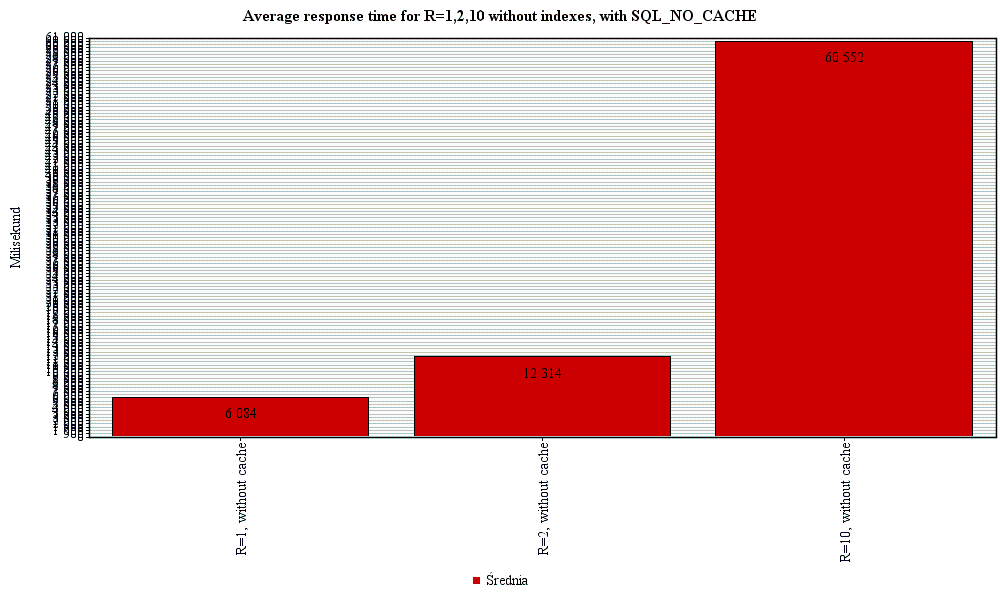
\includegraphics[width=1.15\textwidth]{./avrg_without_indexes}~\\[1cm]
\begin{tabular}{|c|c||c|}
\hline
R - Rooms & 
S - Number of shows scheduled for room & 
Total number of entities \\
\hline
1 &
10k &
10k \\
\hline
2 &
10k &
20k \\
\hline
5 & 
10k & 
50k \\
\hline 
\end{tabular} 
Where k stands for 1000, M stands for 1000k. 

Without indexes response time is linear to number of asked rooms about. 
\section{Tests with index key, still with SQL\_NO\_CACHE}
In second phase indexes were added to the table in following manner. 

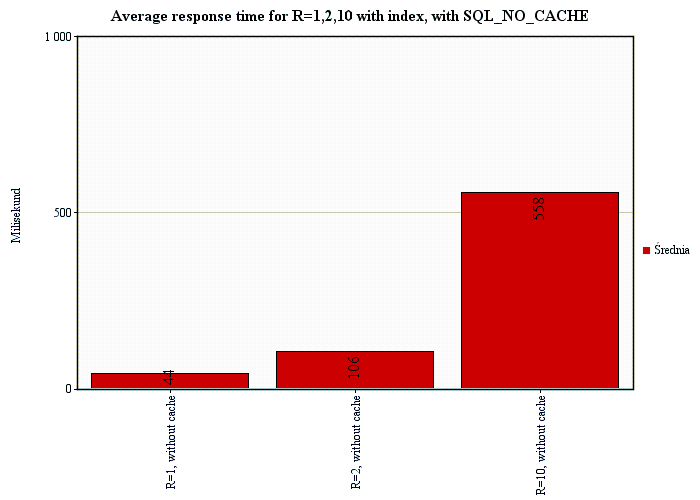
\includegraphics[width=1.15\textwidth]{./avrg_with_indexes}~\\[1cm]
\lstset{language=SQL}
\begin{lstlisting}[frame=single]
ADD PRIMARY KEY (`id`),
ADD INDEX `fk_room_schedule_room1_idx` (`room_id` ASC)
\end{lstlisting}

Table below represents how many entries in each table were added in each phase. 
\begin{tabular}{|c|c||c|}
\hline
R - Rooms & 
S - Number of shows scheduled for room & 
Total number of entities \\
\hline
1 &
10k &
10k \\
\hline
2 &
10k &
20k \\
\hline
5 & 
10k & 
50k \\
\hline 
\end{tabular} 
Where k stands for 1000, M stands for 1000k. 

\section{Comparision without and with an index}
\begin{tabular}{|c|c|c|c|}
\hline
Rooms &
Response time without index [ms] &
 Response time with index [ms] &
Improvement \\
\hline
1 &
6,084 &
44 &
13827\% \\
\hline
2 &
12,314 &
106 &
11617\% \\
\hline
10 &
60,552 &
558 &
10852\% \\
\hline
\end{tabular}
The difference is tremendous.Adding index improved performance even 138 times. 
\section{Measuring importance of caching}
Caching provides saving recent queries and serving them just from memory instead calculating answer from scratch. In order to see cache the same query must be executed few times in “close enough” time. “Close enough” means such a short time, that database server will not purge it’s cache - this may happen if period of time elapsed or specific amount of other queries was executed in between two queries. 
    In order to spot the difference, Apache JMeter was reconfigured in that way, that it makes the same request 4 times in a row. 


% Upper part of the page. The '~' is needed because \\
% only works if a paragraph has started.
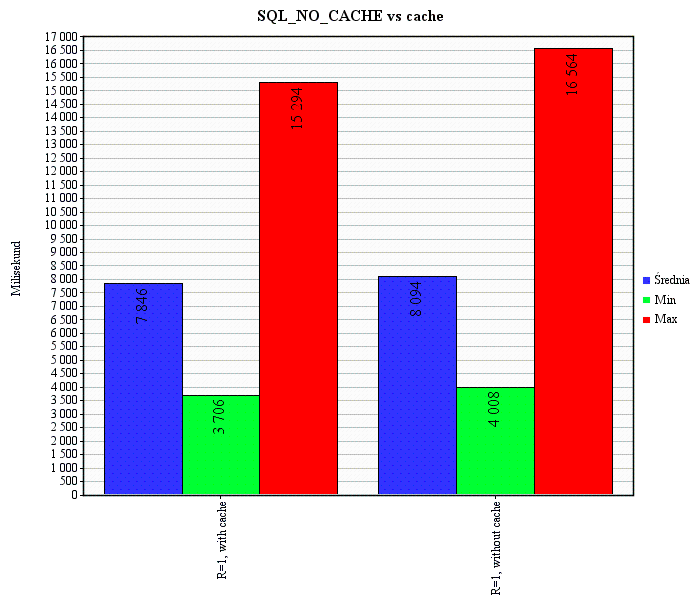
\includegraphics[width=1.15\textwidth]{./cache_vs_nocache}~\\[1cm]

\begin{tabular}{|c|c|c|c|}
\hline
& 
Without cache &
With cache \\
\hline
Mean &
8,094 &
7,846 \\
\hline

Min &
4408 & 
3,706 \\
\hline
Max &
16564 &
15294 \\
\end{tabular}

Applying cache slightly improves performance. Average response time dropped down a little (by 200ms), and minimum response time decreased from 4,4s to 3,7s. 


\end{document}